% 图 44.2 —— 由 `checks/emit_hand.py` 自动拼出（probe 精测 + prims2 图元分解）
%%
% ⚠ 这是**稿子不是成品**：跑 `checks/checkhand.py 44.2` 看指标 + 看叠合图。
%%
%% ⚠ 待核：
%   · 本图 probe 报出阴影族 1 个 —— **本脚本不生成阴影**（要照原书手写）；prims2 的 strokes 里可能含阴影线，核对时留意别画重
%   · 可疑字形 1 项（空心圈 ⊙ 常被认成字母 o）—— 见文件末
%%
\documentclass[12pt]{standalone}
\usepackage{fontspec}
\setsansfont{Arial}
\newfontfamily\mfallback{DejaVu Sans}
\usepackage{tikz}
\begin{document}
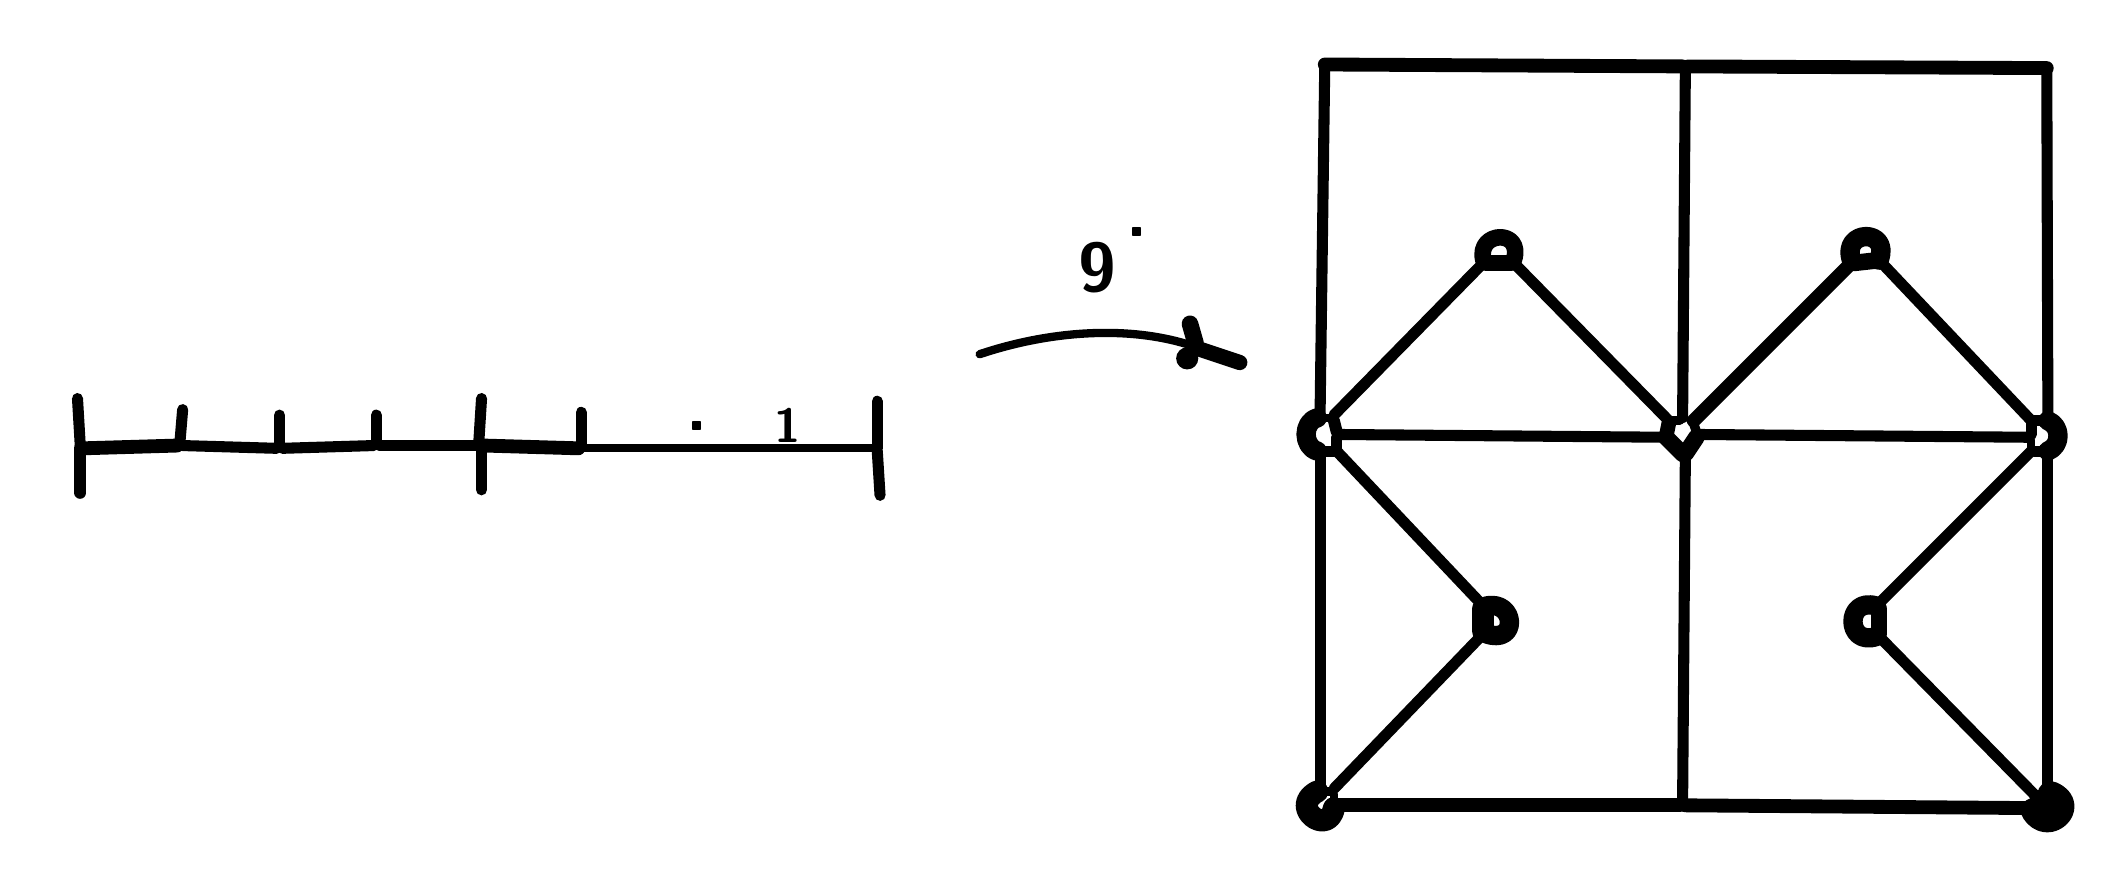
\begin{tikzpicture}[x=1pt, y=-1pt, line width=4.0pt, line cap=round, line join=round]

  %% ════ 填充区（prims2 的 fills）════

  %% ════ 直线段（prims2 的 strokes）════
  \draw[line width=4.0pt] (162.0,151.0) -- (127.0,151.0);
  \draw[line width=5.0pt] (473.0,281.0) -- (597.0,281.0);
  \draw[line width=6.0pt] (669.0,210.0) -- (669.0,219.0);
  \draw[line width=4.0pt] (537.0,85.0) -- (593.0,142.0);
  \draw[line width=4.0pt] (164.0,167.0) -- (164.0,152.0);
  \draw[line width=4.0pt] (90.0,152.0) -- (56.0,151.0);
  \draw[line width=4.0pt] (472.0,275.0) -- (526.0,219.0);
  \draw[line width=4.0pt] (725.0,277.0) -- (669.0,220.0);
  \draw[line width=4.0pt] (473.0,153.0) -- (526.0,209.0);
  \draw[line width=4.0pt] (91.0,140.0) -- (91.0,151.0);
  \draw[line width=6.0pt] (669.0,84.0) -- (660.0,85.0);
  \draw[line width=4.0pt] (669.0,84.0) -- (724.0,142.0);
  \draw[line width=4.0pt] (730.0,141.0) -- (729.6,14.6);
  \draw[line width=5.0pt] (729.6,14.6) -- (600.0,14.0);
  \draw[line width=4.0pt] (729.0,142.0) -- (725.0,142.0);
  \draw[line width=4.0pt] (729.0,153.0) -- (725.0,153.0);
  \draw[line width=4.5pt] (19.0,152.0) -- (19.0,168.0);
  \draw[line width=5.0pt] (598.0,14.0) -- (468.7,13.3);
  \draw[line width=4.0pt] (468.7,13.3) -- (467.0,140.0);
  \draw[line width=4.0pt] (730.0,154.0) -- (730.0,276.0);
  \draw[line width=4.0pt] (599.0,15.0) -- (598.0,141.0);
  \draw[line width=3.0pt] (594.0,142.0) -- (597.0,142.0);
  \draw[line width=4.0pt] (467.0,154.0) -- (467.0,275.0);
  \draw[line width=4.0pt] (307.0,135.0) -- (307.0,152.0);
  \draw[line width=4.0pt] (468.0,153.0) -- (472.0,153.0);
  \draw[line width=3.0pt] (729.0,277.0) -- (726.0,277.0);
  \draw[line width=4.0pt] (724.0,153.0) -- (669.0,208.0);
  \draw[line width=4.0pt] (599.0,155.0) -- (598.0,280.0);
  \draw[line width=4.0pt] (18.0,134.0) -- (19.0,151.0);
  \draw[line width=4.0pt] (125.0,151.0) -- (92.0,152.0);
  \draw[line width=8.0pt] (526.0,218.0) -- (526.0,210.0);
  \draw[line width=6.0pt] (527.0,85.0) -- (536.0,85.0);
  \draw[line width=5.0pt] (199.0,152.0) -- (165.0,151.0);
  \draw[line width=4.0pt] (472.0,140.0) -- (526.0,85.0);
  \draw[line width=4.0pt] (723.0,148.0) -- (604.0,147.0);
  \draw[line width=5.0pt] (54.0,151.0) -- (20.0,152.0);
  \draw[line width=4.0pt] (200.0,151.0) -- (200.0,139.0);
  \draw[line width=4.3pt] (472.0,142.0) -- (473.0,146.0);
  \draw[line width=4.0pt] (724.0,147.0) -- (724.0,143.0);
  \draw[line width=3.0pt] (724.0,149.0) -- (724.0,152.0);
  \draw[line width=3.0pt] (472.0,280.0) -- (472.0,277.0);
  \draw[line width=3.0pt] (468.0,276.0) -- (471.0,276.0);
  \draw[line width=4.0pt] (163.0,150.0) -- (164.0,134.0);
  \draw[line width=5.5pt] (438.0,121.0) -- (423.0,116.0);
  \draw[line width=3.0pt] (471.0,141.0) -- (468.0,141.0);
  \draw[line width=4.0pt] (126.0,150.0) -- (126.0,140.0);
  \draw[line width=3.0pt] (306.0,152.0) -- (201.0,152.0);
  \draw[line width=5.3pt] (592.0,148.0) -- (593.0,143.0);
  \draw[line width=4.0pt] (592.0,148.0) -- (474.0,147.0);
  \draw[line width=6.0pt] (592.0,148.0) -- (598.0,154.0);
  \draw[line width=6.0pt] (420.0,107.0) -- (422.0,114.0);
  \draw[line width=6.0pt] (599.0,154.0) -- (603.0,148.0);
  \draw[line width=4.0pt] (55.0,150.0) -- (56.0,138.0);
  \draw[line width=4.0pt] (473.0,152.0) -- (473.0,148.0);
  \draw[line width=4.0pt] (307.0,153.0) -- (308.0,169.0);
  \draw[line width=3.0pt] (725.0,278.0) -- (725.0,281.0);
  \draw[line width=5.0pt] (602.0,142.0) -- (659.0,85.0);
  \draw[line width=5.0pt] (724.0,282.0) -- (599.0,281.0);
  \draw[line width=3.4pt] (602.0,143.0) -- (603.0,146.0);

  %% ════ 曲线（prims2 的 curves —— 三段式，坐标同为 (y,x)）════
  \draw[line width=7.0pt] (527.0,209.0) .. controls (537.7,206.6) and (538.8,223.2) .. (527.0,219.0);
  \draw[line width=7.0pt] (669.0,84.0) .. controls (673.4,72.5) and (655.3,72.8) .. (659.0,84.0);
  \draw[line width=9.5pt] (725.0,283.0) .. controls (730.1,291.1) and (740.5,280.8) .. (731.0,277.0);
  \draw[line width=7.0pt] (466.0,153.0) .. controls (460.6,151.4) and (460.6,142.4) .. (466.0,141.0);
  \draw[line width=8.0pt] (466.0,276.0) .. controls (455.4,281.5) and (470.0,292.7) .. (472.0,282.0);
  \draw[line width=7.0pt] (668.0,209.0) .. controls (656.7,205.5) and (656.8,223.7) .. (668.0,220.0);
  \draw[line width=7.0pt] (730.0,153.0) .. controls (734.9,151.1) and (734.9,143.9) .. (730.0,142.0);
  \draw[line width=6.0pt] (526.0,84.0) .. controls (523.4,73.4) and (540.7,72.6) .. (537.0,84.0);
  \draw[line width=3.0pt] (344.0,118.0) .. controls (367.7,110.0) and (396.8,107.0) .. (421.0,115.0);

  %% ════ 实心点 ════
  \fill (419.0,119.5) circle (4.0);

  %% ════ 标签（probe 直接给的 \node 行）════
  %% ⚠ 全部补了 fill=white：文字在最上层，否则与曲线交叉干扰
     \node[anchor=center,inner sep=0pt,fill=white,font=\fontsize{39.7}{49.6}\selectfont] at (401.0,73.8) {\textsf{\textbf{.}}};   % box(396,70,4,7)
     \node[anchor=center,inner sep=0pt,fill=white,font=\fontsize{33.1}{41.3}\selectfont] at (386.4,86.8) {\textsf{\textbf{9}}};   % box(376,75,17,22)
     \node[anchor=center,inner sep=0pt,fill=white,font=\fontsize{66.2}{82.8}\selectfont] at (242.0,144.1) {\textsf{\textbf{.}}};   % box(234,137,6,13)
     \node[anchor=center,inner sep=0pt,fill=white,font=\fontsize{16.9}{21.2}\selectfont] at (274.5,143.8) {\textsf{\textbf{1}}};   % box(270,137,5,13)

  % 钉死画布：否则超出的图元/控制点会把页面撑大，1:1 回比就失准
  \pgfresetboundingbox
  \path[use as bounding box] (0,0) rectangle (748,298);
\end{tikzpicture}
\end{document}

% ⚠ 待核清单（probe 拿不准，人眼过一遍）：
%   · 未识别/跳过：⑤ 跳过/未识别的字形
